\documentclass{standalone}
\usepackage{tikz}
\usetikzlibrary{patterns, positioning}

\begin{document}
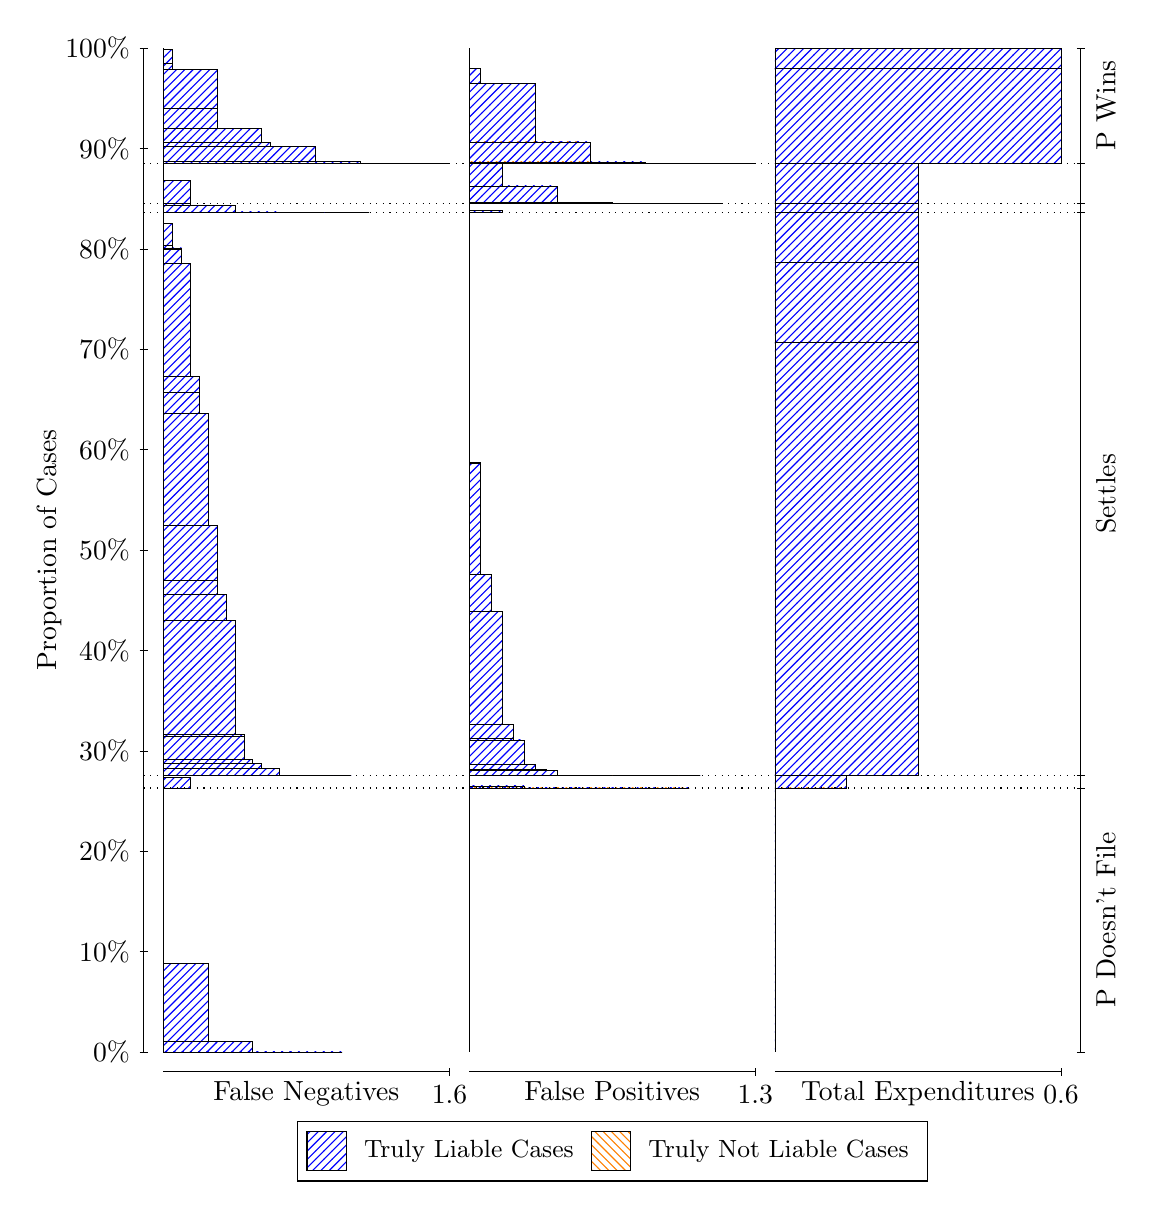
\begin{tikzpicture}
\draw[black, very thin] (1.5,1.75) -- (1.5,14.5);
\node[rotate=90, anchor=center] at (0.3, 8.125) {Proportion of Cases};
\draw[black, very thin] (1.45,1.75) -- (1.55,1.75);
\node[anchor=east] at (1.45, 1.75) {0\%};
\draw[black, very thin] (1.45,3.025) -- (1.55,3.025);
\node[anchor=east] at (1.45, 3.025) {10\%};
\draw[black, very thin] (1.45,4.3) -- (1.55,4.3);
\node[anchor=east] at (1.45, 4.3) {20\%};
\draw[black, very thin] (1.45,5.575) -- (1.55,5.575);
\node[anchor=east] at (1.45, 5.575) {30\%};
\draw[black, very thin] (1.45,6.85) -- (1.55,6.85);
\node[anchor=east] at (1.45, 6.85) {40\%};
\draw[black, very thin] (1.45,8.125) -- (1.55,8.125);
\node[anchor=east] at (1.45, 8.125) {50\%};
\draw[black, very thin] (1.45,9.4) -- (1.55,9.4);
\node[anchor=east] at (1.45, 9.4) {60\%};
\draw[black, very thin] (1.45,10.675) -- (1.55,10.675);
\node[anchor=east] at (1.45, 10.675) {70\%};
\draw[black, very thin] (1.45,11.95) -- (1.55,11.95);
\node[anchor=east] at (1.45, 11.95) {80\%};
\draw[black, very thin] (1.45,13.225) -- (1.55,13.225);
\node[anchor=east] at (1.45, 13.225) {90\%};
\draw[black, very thin] (1.45,14.5) -- (1.55,14.5);
\node[anchor=east] at (1.45, 14.5) {100\%};

\draw[black, very thin] (13.4,1.75) -- (13.4,14.5);
\draw[black, very thin] (13.35,1.75) -- (13.45,1.75);
\node[anchor=west] at (13.35, 1.75) {};
\draw[black, very thin] (13.35,5.103) -- (13.45,5.103);
\node[anchor=west] at (13.35, 5.103) {};
\draw[black, very thin] (13.35,5.2663) -- (13.45,5.2663);
\node[anchor=west] at (13.35, 5.2663) {};
\draw[black, very thin] (13.35,12.409) -- (13.45,12.409);
\node[anchor=west] at (13.35, 12.409) {};
\draw[black, very thin] (13.35,12.529) -- (13.45,12.529);
\node[anchor=west] at (13.35, 12.529) {};
\draw[black, very thin] (13.35,13.036) -- (13.45,13.036);
\node[anchor=west] at (13.35, 13.036) {};
\draw[black, very thin] (13.35,14.5) -- (13.45,14.5);
\node[anchor=west] at (13.35, 14.5) {};

\draw[black, very thin, pattern color=blue, pattern=north east lines] (1.75,1.75) rectangle (4.0208,1.75);
\draw[black, very thin, pattern color=blue, pattern=north east lines] (1.75,1.75) rectangle (3.4531,1.7512);
\draw[black, very thin, pattern color=blue, pattern=north east lines] (1.75,1.7512) rectangle (2.8854,1.8889);
\draw[black, very thin, pattern color=blue, pattern=north east lines] (1.75,1.8889) rectangle (2.3177,2.8742);
\draw[black, very thin, pattern color=orange, pattern=north west lines] (1.75,2.8742) rectangle (1.75,2.8742);
\draw[black, very thin, pattern color=blue, pattern=north east lines] (1.75,2.8742) rectangle (1.75,5.103);
\draw[black, very thin, pattern color=blue, pattern=north east lines] (1.75,5.103) rectangle (2.0906,5.2396);
\draw[black, very thin, pattern color=orange, pattern=north west lines] (1.75,5.2396) rectangle (1.75,5.2396);
\draw[black, very thin, pattern color=blue, pattern=north east lines] (1.75,5.2396) rectangle (1.75,5.2663);
\draw[black, very thin, pattern color=blue, pattern=north east lines] (1.75,5.2663) rectangle (4.1344,5.2663);
\draw[black, very thin, pattern color=blue, pattern=north east lines] (1.75,5.2663) rectangle (3.9073,5.2663);
\draw[black, very thin, pattern color=blue, pattern=north east lines] (1.75,5.2663) rectangle (3.6802,5.2663);
\draw[black, very thin, pattern color=blue, pattern=north east lines] (1.75,5.2663) rectangle (3.5667,5.2663);
\draw[black, very thin, pattern color=blue, pattern=north east lines] (1.75,5.2663) rectangle (3.4531,5.2664);
\draw[black, very thin, pattern color=blue, pattern=north east lines] (1.75,5.2664) rectangle (3.3396,5.2665);
\draw[black, very thin, pattern color=blue, pattern=north east lines] (1.75,5.2665) rectangle (3.226,5.3479);
\draw[black, very thin, pattern color=blue, pattern=north east lines] (1.75,5.3479) rectangle (3.1125,5.3506);
\draw[black, very thin, pattern color=blue, pattern=north east lines] (1.75,5.3506) rectangle (2.999,5.4189);
\draw[black, very thin, pattern color=blue, pattern=north east lines] (1.75,5.4189) rectangle (2.8854,5.4625);
\draw[black, very thin, pattern color=blue, pattern=north east lines] (1.75,5.4625) rectangle (2.7719,5.7575);
\draw[black, very thin, pattern color=blue, pattern=north east lines] (1.75,5.7575) rectangle (2.7719,5.7797);
\draw[black, very thin, pattern color=blue, pattern=north east lines] (1.75,5.7797) rectangle (2.6583,7.2348);
\draw[black, very thin, pattern color=blue, pattern=north east lines] (1.75,7.2348) rectangle (2.5448,7.5587);
\draw[black, very thin, pattern color=blue, pattern=north east lines] (1.75,7.5587) rectangle (2.4312,7.7383);
\draw[black, very thin, pattern color=blue, pattern=north east lines] (1.75,7.7383) rectangle (2.4312,8.438);
\draw[black, very thin, pattern color=blue, pattern=north east lines] (1.75,8.438) rectangle (2.3177,9.8634);
\draw[black, very thin, pattern color=blue, pattern=north east lines] (1.75,9.8634) rectangle (2.2042,10.124);
\draw[black, very thin, pattern color=blue, pattern=north east lines] (1.75,10.124) rectangle (2.2042,10.327);
\draw[black, very thin, pattern color=blue, pattern=north east lines] (1.75,10.327) rectangle (2.0906,11.767);
\draw[black, very thin, pattern color=blue, pattern=north east lines] (1.75,11.767) rectangle (1.9771,11.943);
\draw[black, very thin, pattern color=blue, pattern=north east lines] (1.75,11.943) rectangle (1.9771,11.961);
\draw[black, very thin, pattern color=blue, pattern=north east lines] (1.75,11.961) rectangle (1.8635,11.994);
\draw[black, very thin, pattern color=blue, pattern=north east lines] (1.75,11.994) rectangle (1.8635,12.269);
\draw[black, very thin, pattern color=blue, pattern=north east lines] (1.75,12.269) rectangle (1.75,12.269);
\draw[black, very thin, pattern color=orange, pattern=north west lines] (1.75,12.269) rectangle (1.75,12.269);
\draw[black, very thin, pattern color=blue, pattern=north east lines] (1.75,12.269) rectangle (1.75,12.409);
\draw[black, very thin, pattern color=blue, pattern=north east lines] (1.75,12.409) rectangle (4.3615,12.409);
\draw[black, very thin, pattern color=blue, pattern=north east lines] (1.75,12.409) rectangle (3.7937,12.409);
\draw[black, very thin, pattern color=blue, pattern=north east lines] (1.75,12.409) rectangle (3.226,12.419);
\draw[black, very thin, pattern color=blue, pattern=north east lines] (1.75,12.419) rectangle (2.6583,12.502);
\draw[black, very thin, pattern color=blue, pattern=north east lines] (1.75,12.502) rectangle (2.0906,12.529);
\draw[black, very thin, pattern color=orange, pattern=north west lines] (1.75,12.529) rectangle (1.75,12.529);
\draw[black, very thin, pattern color=blue, pattern=north east lines] (1.75,12.529) rectangle (2.0906,12.817);
\draw[black, very thin, pattern color=orange, pattern=north west lines] (1.75,12.817) rectangle (1.75,12.817);
\draw[black, very thin, pattern color=blue, pattern=north east lines] (1.75,12.817) rectangle (1.75,13.036);
\draw[black, very thin, pattern color=blue, pattern=north east lines] (1.75,13.036) rectangle (5.3833,13.036);
\draw[black, very thin, pattern color=blue, pattern=north east lines] (1.75,13.036) rectangle (4.8156,13.036);
\draw[black, very thin, pattern color=blue, pattern=north east lines] (1.75,13.036) rectangle (4.2479,13.063);
\draw[black, very thin, pattern color=blue, pattern=north east lines] (1.75,13.063) rectangle (4.1344,13.063);
\draw[black, very thin, pattern color=blue, pattern=north east lines] (1.75,13.063) rectangle (3.6802,13.247);
\draw[black, very thin, pattern color=blue, pattern=north east lines] (1.75,13.247) rectangle (3.5667,13.249);
\draw[black, very thin, pattern color=blue, pattern=north east lines] (1.75,13.249) rectangle (3.1125,13.298);
\draw[black, very thin, pattern color=blue, pattern=north east lines] (1.75,13.298) rectangle (2.999,13.481);
\draw[black, very thin, pattern color=blue, pattern=north east lines] (1.75,13.481) rectangle (2.5448,13.482);
\draw[black, very thin, pattern color=blue, pattern=north east lines] (1.75,13.482) rectangle (2.4312,13.732);
\draw[black, very thin, pattern color=blue, pattern=north east lines] (1.75,13.732) rectangle (2.4312,14.229);
\draw[black, very thin, pattern color=blue, pattern=north east lines] (1.75,14.229) rectangle (1.9771,14.229);
\draw[black, very thin, pattern color=blue, pattern=north east lines] (1.75,14.229) rectangle (1.8635,14.3);
\draw[black, very thin, pattern color=blue, pattern=north east lines] (1.75,14.3) rectangle (1.8635,14.482);
\draw[black, very thin, pattern color=orange, pattern=north west lines] (1.75,14.482) rectangle (1.75,14.482);
\draw[black, very thin, pattern color=blue, pattern=north east lines] (1.75,14.482) rectangle (1.75,14.5);
\draw[black, very thin, pattern color=orange, pattern=north west lines] (5.6333,1.75) rectangle (5.6333,1.75);
\draw[black, very thin, pattern color=blue, pattern=north east lines] (5.6333,1.75) rectangle (5.6333,5.103);
\draw[black, very thin, pattern color=orange, pattern=north west lines] (5.6333,5.103) rectangle (8.4282,5.103);
\draw[black, very thin, pattern color=blue, pattern=north east lines] (5.6333,5.103) rectangle (8.4282,5.103);
\draw[black, very thin, pattern color=blue, pattern=north east lines] (5.6333,5.103) rectangle (7.7295,5.103);
\draw[black, very thin, pattern color=blue, pattern=north east lines] (5.6333,5.103) rectangle (7.0308,5.1032);
\draw[black, very thin, pattern color=blue, pattern=north east lines] (5.6333,5.1032) rectangle (6.3321,5.1297);
\draw[black, very thin, pattern color=blue, pattern=north east lines] (5.6333,5.1297) rectangle (5.6333,5.2663);
\draw[black, very thin, pattern color=orange, pattern=north west lines] (5.6333,5.2663) rectangle (8.5679,5.2663);
\draw[black, very thin, pattern color=blue, pattern=north east lines] (5.6333,5.2663) rectangle (8.5679,5.2663);
\draw[black, very thin, pattern color=orange, pattern=north west lines] (5.6333,5.2663) rectangle (8.2885,5.2663);
\draw[black, very thin, pattern color=blue, pattern=north east lines] (5.6333,5.2663) rectangle (8.2885,5.2663);
\draw[black, very thin, pattern color=orange, pattern=north west lines] (5.6333,5.2663) rectangle (8.009,5.2663);
\draw[black, very thin, pattern color=blue, pattern=north east lines] (5.6333,5.2663) rectangle (8.009,5.2663);
\draw[black, very thin, pattern color=blue, pattern=north east lines] (5.6333,5.2663) rectangle (7.8692,5.2663);
\draw[black, very thin, pattern color=orange, pattern=north west lines] (5.6333,5.2663) rectangle (7.7295,5.2663);
\draw[black, very thin, pattern color=blue, pattern=north east lines] (5.6333,5.2663) rectangle (7.7295,5.2663);
\draw[black, very thin, pattern color=blue, pattern=north east lines] (5.6333,5.2663) rectangle (7.5897,5.2663);
\draw[black, very thin, pattern color=orange, pattern=north west lines] (5.6333,5.2663) rectangle (7.45,5.2663);
\draw[black, very thin, pattern color=blue, pattern=north east lines] (5.6333,5.2663) rectangle (7.45,5.2663);
\draw[black, very thin, pattern color=blue, pattern=north east lines] (5.6333,5.2663) rectangle (7.3103,5.2663);
\draw[black, very thin, pattern color=orange, pattern=north west lines] (5.6333,5.2663) rectangle (7.1705,5.2663);
\draw[black, very thin, pattern color=blue, pattern=north east lines] (5.6333,5.2663) rectangle (7.1705,5.2663);
\draw[black, very thin, pattern color=orange, pattern=north west lines] (5.6333,5.2663) rectangle (7.1705,5.2663);
\draw[black, very thin, pattern color=blue, pattern=north east lines] (5.6333,5.2663) rectangle (7.1705,5.2663);
\draw[black, very thin, pattern color=blue, pattern=north east lines] (5.6333,5.2663) rectangle (7.0308,5.2664);
\draw[black, very thin, pattern color=blue, pattern=north east lines] (5.6333,5.2664) rectangle (6.891,5.2665);
\draw[black, very thin, pattern color=orange, pattern=north west lines] (5.6333,5.2665) rectangle (6.891,5.2665);
\draw[black, very thin, pattern color=blue, pattern=north east lines] (5.6333,5.2665) rectangle (6.891,5.2675);
\draw[black, very thin, pattern color=blue, pattern=north east lines] (5.6333,5.2675) rectangle (6.7513,5.3214);
\draw[black, very thin, pattern color=orange, pattern=north west lines] (5.6333,5.3214) rectangle (6.6115,5.3214);
\draw[black, very thin, pattern color=blue, pattern=north east lines] (5.6333,5.3214) rectangle (6.6115,5.3403);
\draw[black, very thin, pattern color=blue, pattern=north east lines] (5.6333,5.3403) rectangle (6.4718,5.4059);
\draw[black, very thin, pattern color=blue, pattern=north east lines] (5.6333,5.4059) rectangle (6.4718,5.4061);
\draw[black, very thin, pattern color=orange, pattern=north west lines] (5.6333,5.4061) rectangle (6.3321,5.4061);
\draw[black, very thin, pattern color=blue, pattern=north east lines] (5.6333,5.4061) rectangle (6.3321,5.7141);
\draw[black, very thin, pattern color=blue, pattern=north east lines] (5.6333,5.7141) rectangle (6.1923,5.7321);
\draw[black, very thin, pattern color=blue, pattern=north east lines] (5.6333,5.7321) rectangle (6.1923,5.9077);
\draw[black, very thin, pattern color=blue, pattern=north east lines] (5.6333,5.9077) rectangle (6.0526,7.3482);
\draw[black, very thin, pattern color=blue, pattern=north east lines] (5.6333,7.3482) rectangle (5.9128,7.8115);
\draw[black, very thin, pattern color=blue, pattern=north east lines] (5.6333,7.8115) rectangle (5.7731,9.2326);
\draw[black, very thin, pattern color=blue, pattern=north east lines] (5.6333,9.2326) rectangle (5.7731,9.2369);
\draw[black, very thin, pattern color=blue, pattern=north east lines] (5.6333,9.2369) rectangle (5.6333,12.409);
\draw[black, very thin, pattern color=orange, pattern=north west lines] (5.6333,12.409) rectangle (6.0526,12.409);
\draw[black, very thin, pattern color=blue, pattern=north east lines] (5.6333,12.409) rectangle (6.0526,12.435);
\draw[black, very thin, pattern color=blue, pattern=north east lines] (5.6333,12.435) rectangle (5.6333,12.529);
\draw[black, very thin, pattern color=orange, pattern=north west lines] (5.6333,12.529) rectangle (8.8474,12.529);
\draw[black, very thin, pattern color=blue, pattern=north east lines] (5.6333,12.529) rectangle (8.8474,12.529);
\draw[black, very thin, pattern color=blue, pattern=north east lines] (5.6333,12.529) rectangle (8.1487,12.529);
\draw[black, very thin, pattern color=blue, pattern=north east lines] (5.6333,12.529) rectangle (7.45,12.536);
\draw[black, very thin, pattern color=blue, pattern=north east lines] (5.6333,12.536) rectangle (6.7513,12.748);
\draw[black, very thin, pattern color=blue, pattern=north east lines] (5.6333,12.748) rectangle (6.0526,13.036);
\draw[black, very thin, pattern color=orange, pattern=north west lines] (5.6333,13.036) rectangle (9.2667,13.036);
\draw[black, very thin, pattern color=blue, pattern=north east lines] (5.6333,13.036) rectangle (9.2667,13.036);
\draw[black, very thin, pattern color=orange, pattern=north west lines] (5.6333,13.036) rectangle (8.5679,13.036);
\draw[black, very thin, pattern color=blue, pattern=north east lines] (5.6333,13.036) rectangle (8.5679,13.036);
\draw[black, very thin, pattern color=orange, pattern=north west lines] (5.6333,13.036) rectangle (7.8692,13.036);
\draw[black, very thin, pattern color=blue, pattern=north east lines] (5.6333,13.036) rectangle (7.8692,13.054);
\draw[black, very thin, pattern color=orange, pattern=north west lines] (5.6333,13.054) rectangle (7.1705,13.054);
\draw[black, very thin, pattern color=blue, pattern=north east lines] (5.6333,13.054) rectangle (7.1705,13.307);
\draw[black, very thin, pattern color=orange, pattern=north west lines] (5.6333,13.307) rectangle (7.0308,13.307);
\draw[black, very thin, pattern color=blue, pattern=north east lines] (5.6333,13.307) rectangle (7.0308,13.307);
\draw[black, very thin, pattern color=blue, pattern=north east lines] (5.6333,13.307) rectangle (6.4718,14.054);
\draw[black, very thin, pattern color=orange, pattern=north west lines] (5.6333,14.054) rectangle (6.3321,14.054);
\draw[black, very thin, pattern color=blue, pattern=north east lines] (5.6333,14.054) rectangle (6.3321,14.054);
\draw[black, very thin, pattern color=blue, pattern=north east lines] (5.6333,14.054) rectangle (5.7731,14.238);
\draw[black, very thin, pattern color=orange, pattern=north west lines] (5.6333,14.238) rectangle (5.6333,14.238);
\draw[black, very thin, pattern color=blue, pattern=north east lines] (5.6333,14.238) rectangle (5.6333,14.5);
\draw[black, very thin, pattern color=orange, pattern=north west lines] (9.5167,1.75) rectangle (9.5167,1.75);
\draw[black, very thin, pattern color=blue, pattern=north east lines] (9.5167,1.75) rectangle (9.5167,5.103);
\draw[black, very thin, pattern color=orange, pattern=north west lines] (9.5167,5.103) rectangle (10.425,5.103);
\draw[black, very thin, pattern color=blue, pattern=north east lines] (9.5167,5.103) rectangle (10.425,5.2663);
\draw[black, very thin, pattern color=orange, pattern=north west lines] (9.5167,5.2663) rectangle (11.333,5.2663);
\draw[black, very thin, pattern color=blue, pattern=north east lines] (9.5167,5.2663) rectangle (11.333,10.769);
\draw[black, very thin, pattern color=orange, pattern=north west lines] (9.5167,10.769) rectangle (11.333,10.769);
\draw[black, very thin, pattern color=blue, pattern=north east lines] (9.5167,10.769) rectangle (11.333,11.773);
\draw[black, very thin, pattern color=orange, pattern=north west lines] (9.5167,11.773) rectangle (11.333,11.773);
\draw[black, very thin, pattern color=blue, pattern=north east lines] (9.5167,11.773) rectangle (11.333,12.409);
\draw[black, very thin, pattern color=orange, pattern=north west lines] (9.5167,12.409) rectangle (11.333,12.409);
\draw[black, very thin, pattern color=blue, pattern=north east lines] (9.5167,12.409) rectangle (11.333,12.529);
\draw[black, very thin, pattern color=orange, pattern=north west lines] (9.5167,12.529) rectangle (11.333,12.529);
\draw[black, very thin, pattern color=blue, pattern=north east lines] (9.5167,12.529) rectangle (11.333,13.036);
\draw[black, very thin, pattern color=orange, pattern=north west lines] (9.5167,13.036) rectangle (13.15,13.036);
\draw[black, very thin, pattern color=blue, pattern=north east lines] (9.5167,13.036) rectangle (13.15,14.24);
\draw[black, very thin, pattern color=orange, pattern=north west lines] (9.5167,14.24) rectangle (13.15,14.24);
\draw[black, very thin, pattern color=blue, pattern=north east lines] (9.5167,14.24) rectangle (13.15,14.5);
\draw[black, dotted] (1.5,5.103) -- (13.4,5.103);
\draw[black, dotted] (1.5,5.2663) -- (13.4,5.2663);
\draw[black, dotted] (1.5,12.409) -- (13.4,12.409);
\draw[black, dotted] (1.5,12.529) -- (13.4,12.529);
\draw[black, dotted] (1.5,13.036) -- (13.4,13.036);
\draw[black, very thin] (1.75,1.5) -- (5.3833,1.5);
\node[anchor=north] at (3.5667, 1.5) {False Negatives};
\draw[black, very thin] (5.3833,1.45) -- (5.3833,1.55);
\node[anchor=north] at (5.3833, 1.45) {1.6};

\draw[black, very thin] (5.6333,1.5) -- (9.2667,1.5);
\node[anchor=north] at (7.45, 1.5) {False Positives};
\draw[black, very thin] (9.2667,1.45) -- (9.2667,1.55);
\node[anchor=north] at (9.2667, 1.45) {1.3};

\draw[black, very thin] (9.5167,1.5) -- (13.15,1.5);
\node[anchor=north] at (11.333, 1.5) {Total Expenditures};
\draw[black, very thin] (13.15,1.45) -- (13.15,1.55);
\node[anchor=north] at (13.15, 1.45) {0.6};

\node[black, centered, rotate=90] at (13.72, 3.4265) {P Doesn't File};

\node[black, centered, rotate=90] at (13.72, 8.8374) {Settles};


\node[black, centered, rotate=90] at (13.72, 13.768) {P Wins};

\draw (7.449999999999999,1.5) node[draw=none] (baseCoordinate) {};
\begin{scope}[align=center]
        \matrix[scale=0.5, draw=black, below=0.5cm of baseCoordinate, nodes={draw}, column sep=0.1cm]{
            \node[rectangle, draw, minimum width=0.5cm, minimum height=0.5cm, pattern=north east lines, pattern color=blue] {}; &
            \node[draw=none, font=\small] (B) {Truly Liable Cases}; &
            \node[rectangle, draw, minimum width=0.5cm, minimum height=0.5cm, pattern=north west lines, pattern color=orange] {}; &
            \node[draw=none, font=\small] (B) {Truly Not Liable Cases}; \\
            };
\end{scope}

\end{tikzpicture}
\end{document}